\begin{figure}[htbp]
    \captionsetup[subfigure]{justification=centering}
    \centering
    \begin{subfigure}[b]{0.25\textwidth} % Decreased width to add space
        \centering
        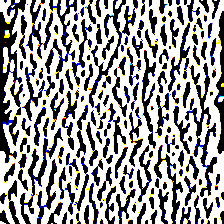
\includegraphics[width=\textwidth]{figures/featurelayersviz/low_channel.png}
        \caption{Lower Level Features}
    \end{subfigure}
    \hspace{0.05\textwidth} % Add space between subfigures
    \begin{subfigure}[b]{0.25\textwidth} % Decreased width to add space
        \centering
        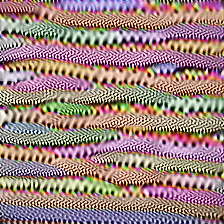
\includegraphics[width=\textwidth]{figures/featurelayersviz/medium_channel.png}
        \caption{Mid Level Features}
    \end{subfigure}
    \hspace{0.05\textwidth} % Add space between subfigures
    \begin{subfigure}[b]{0.25\textwidth} % Decreased width to add space
        \centering
        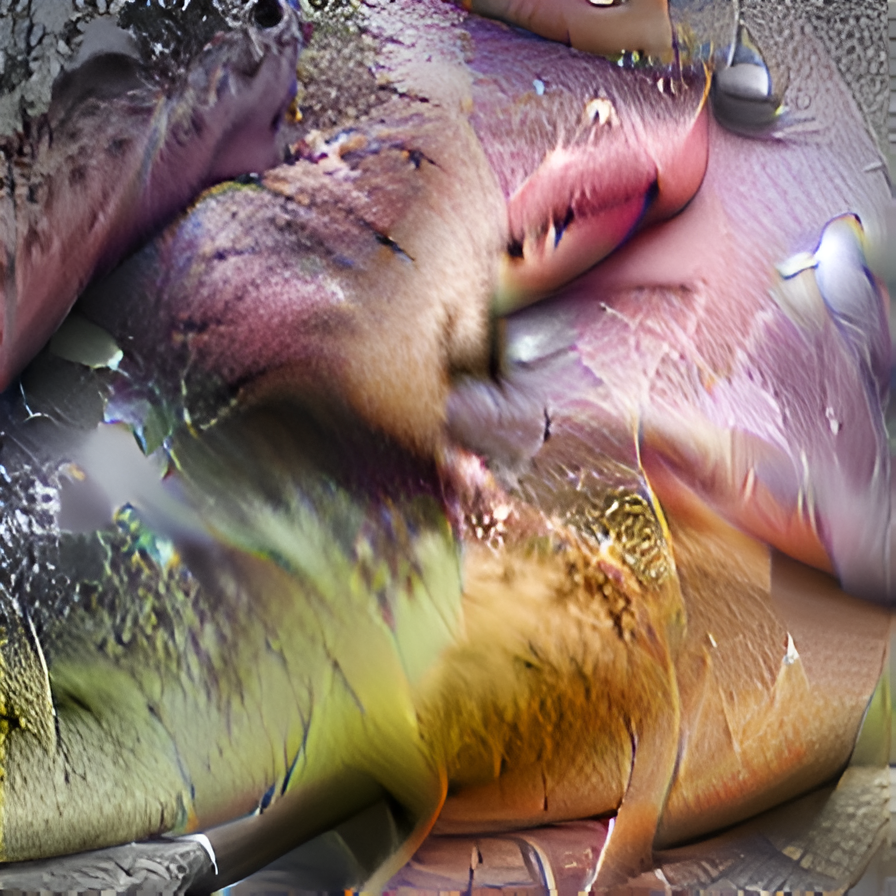
\includegraphics[width=\textwidth]{figures/featurelayersviz/late_channel.png}
        \caption{Higher Level Features}
    \end{subfigure}
    \caption{Illustration of feature representations at different hierarchies. It is visible that lower level features represent 
    more simple structures like edges, whereas higher level features represent complex objects and dependencies. Images taken from \cite{openaifeaturerepres}.}
    \label{fig:featurelayers}
\end{figure}